%
%

\multiproblem{linear}{

    We now consider the equation
    \begin{equation}
        a\,x = b
        \label{eq:axb}
    \end{equation}
    where $a$ and $b$ are known and $x$ is an unknown quantity. We begin by
    knowing that x is from some set say $S$. Equation~\eqref{eq:axb} implies
    that $x$ in fact belongs to a set $T$ which is a subset of $S$
    ($T\subseteq S$).  Our objective is to find the set $T$ comprising all
    solutions of equation~\eqref{eq:axb} for $x\in S$.

    \begin{enumerate}
        \item Let's first consider some examples. What is the solution set
            for $x$ in the following cases?
            \begin{enumerate}
                \item $2\,x = 8$ and $x\in\mathbb{R}$
                \item $0\,x = 8$ and $x\in\mathbb{R}$
                \item $0\,x = 0$ and $x\in\mathbb{R}$
            \end{enumerate}
        \item More generally given $a,b,x\in\mathbb{R}$ how does the solution
            set for~\eqref{eq:axb} depend on $a$ and $b$?
        \item What difference does it make if $a,b,x\in\mathbb{Q}$ or
            $a,b,x\in\mathbb{C}$?
        \item What if $a,b,x\in\mathbb{Z}$?
        \item Consider the same equation in modular arithmetic
            \[
                a\,x = b \Mod{n}
            \]
            with $a,b,x\in\mathbb{Z}$ and $n\in\mathbb{N}$.
            \begin{enumerate}
                \item If $x = 1 \Mod{3}$ what is the solution set for $x$?
                \item If $x = b \Mod{p}$ with $p$ prime what are the sets of
                    solutions for different values of $b$ and $p$?
                \item If $a\,x = b \Mod{p}$ with $p$ prime what are the sets of
                    solutions for different values of $a$ and $b$?
                \item What could happen to the solution set if $p$ is not
                    prime? (consider e.g. $3\,x=3\Mod{6}$ or $3\,x=2\Mod{6})$.
            \end{enumerate}
    \end{enumerate}
}

\multiproblem{quadratic}{
    It's common for mathematical problems to be posed in such a way that the
    number of solutions (the size/cardinality of the solution set) will be
    either $0$, $1$ or $\infty$. When the number of solutions is $0$ we say
    that a solution does not \emph{exist}. If a solution exists but there is
    more than one we say that we do not have a \emph{unique} solution. In many
    areas there will be conditions guaranteeing existence and uniqueness so
    that we can know when there will be exactly one solution.

    The most common exception to the $0,1,\infty$ pattern is when dealing
    with polynomial equations. Here we consider the quadratic equation
    \begin{equation}
        a\,x^2 + b\,x + c = 0.
        \label{eq:quad}
    \end{equation}
    Note that if $a=0$ then this is equivalent to~\eqref{eq:axb}. Often we say
    that by definition a quadratic equation must have $a\neq 0$. In the
    questions below carefully consider how the assumption $a\neq 0$ would
    affect the set of solutions.
    \begin{enumerate}
        \item Given $a,b,c,x\in\mathbb{R}$ what will be the set of solutions
            to~\eqref{eq:quad}? Carefully consider all cases (e.g. $a=0$ or
            perhaps $a=b=0$ but $c\neq 0$ etc.). Under what conditions can we
            guarantee existence or uniqueness of solutions?
        \item What happens to the sets of solutions to~\eqref{eq:quad} if
            $a,b,c,x\in\mathbb{C}$? Under what conditions on $a,b,c$ can we
            guarantee the existence of solutions in this case? (This
            property of complex numbers is called \emph{algebraic closure}.)
        \item Now consider the case that $a,b,c,x\in\mathbb{Z}$. Under what
            conditions do we have existence/uniqueness of solutions?
        \item Given $a,b,c,x\in\mathbb{Z}$ show that if a solution
            to~\eqref{eq:quad} exists then it divides $c$.

            This principle naturally extends to higher-order polynomials so
            show that there are no integer solutions to
            \begin{equation}
                2x^5 - x^4 + 4x^3 - 2x^2 + 2x - 1 = 0
                \label{eq:quintic}
            \end{equation}
        \item Given $a,b,c,x\in\mathbb{Q}$ we can write $a=\frac{n_a}{d_a}$
            etc. and then multiply through by the square of all of the
            denominators to obtain an equation in the same form
            as~\eqref{eq:quad} but with $a,b,c\in\mathbb{Z}$ and
            $x\in\mathbb{Q}$ (prove/verify this).

            Suppose that $a,b,c\in\mathbb{Z}$ and $x\in\mathbb{Q}$ and that
            there exists a rational solution $x=\frac{n}{d}$ (
            $d,n\in\mathbb{Z}$). Show that $n$ divides $c$ and $d$ divides
            $a$.

            How would this generalise to higher order polynomials? Hence find
            the set of all rational solutions to~\eqref{eq:quintic}.
    \end{enumerate}
}

\multiproblem{physics}{
    These next problems will look at sets of solutions in the context of
    simple statics problems. The main things that we need to know from
    physics are Newton's first law for equilibria, Hooke's law ($F=-kx$) for a
    linear spring, and the static friction constraint $F\le\mu N$. Also any
    normal reaction force must satisfy $N\ge 0$.

    (The general principle for answering these questions is to begin by
    drawing a free-body diagram. Then choose coordinate axes and resolve
    forces into components. You can then use Newton's first law, Hooke's law
    and the friction constraint to obtain a system of equations/inequalities
    to be solved mathematically.)

    \begin{enumerate}
        \item Consider the mass spring system shown here:\newline
            \begin{center}
                \includegraphics{mass_horizontal.pdf}
            \end{center}
            The symbols are $g$ the gravitational constant, $m$ the mass of
            the particle, $k,l_0$ the stiffness and natural length of the
            spring, $\mu$ the friction coefficient between the ground and the
            particle, and $x$ the extension of the spring. All quantities
            apart from $x$ are known (even though we won't use numeric values
            for them).

            What is the set of solutions for $x$ satisfying the equilibrium
            conditions in the case that the ground is smooth ($\mu=0$)?

            What happens to the set of solutions in the case that the ground
            is rough?
        \item Now consider a mass on a slope
            \begin{center}
                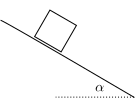
\includegraphics{mass_slope.pdf}
            \end{center}
            at an angle $\alpha$. For what values of $\alpha$ is equilibrium
            possible if the slope is smooth? What if it is rough with
            coefficient $\mu$?
        \item Here we have a mass which is forced against the ground by a
            spring:
            \begin{center}
                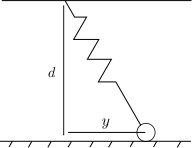
\includegraphics{mass_wall.pdf}
            \end{center}
            We can ignore gravity in this problem.

            Assuming the ground is smooth For what values of $y$ is
            equilibrium possible if $d < l_0$? What if $d = l_0$ or $d > l_0$?
            Sketch the relationship between $y$ and $d$.

            What would happen if the ground was rough?
    \end{enumerate}
}
